% (c) Egor Osipov

\documentclass[a4paper,12pt]{article} % тип документа (report, book)
\usepackage[14pt]{extsizes}
\usepackage[left=2cm,right=2cm, top=2cm,bottom=2cm,bindingoffset=0cm]{geometry} % Настройки документа
\usepackage{pgfplots}
\usepackage{pgfplotstable}
\usepackage{tikz} 

%  Русский язык
\usepackage[T2A]{fontenc}			% кодировка
\usepackage[utf8]{inputenc}			% кодировка исходного текста
\usepackage[english,russian]{babel}	% локализация и переносы


% Математика
\usepackage{amsmath,amsfonts,amssymb,amsthm,mathtools} 

% Просто смайлики
\usepackage{wasysym}

%Вставка картинок
\usepackage{graphicx}
\graphicspath{./}
\DeclareGraphicsExtensions{.pdf,.png,.jpg}
\usepackage{float}

% Настройка абзацев
\usepackage{indentfirst}
%\setlength{\parindent}{5ex}
%\setlength{\parskip}{1em}

\begin{document} % начало документа

%Заговолок
\begin{titlepage}
\begin{center}
	\large{Московский физико-технический институт}\\
	\vspace{100px}
	\LARGE{Лабораторная работа № 3.3.4.}\\
	\LARGE{Эффект Холла в полупроводниках.}\\
	\vspace{30px}
	
\includegraphics[scale = 0.3]{fakt_logo.png}\\
\end{center}

\vfill
\begin{flushright}
	\text{Осипов Егор. Б03-005}\\
	\text{16.11.2021}\\
	\text{г. Долгопрудный}
\end{flushright}
\end{titlepage}

\newpage

\tableofcontents

\newpage

\section{Теория и вводные}

\subsection{Цель работы и используемые приборы.}

\textbf{Цель работы:} измерение подвижности и концентрации носителей заряда в полупроводниках.

\textbf{В работе испольщуются:} электромагнит с источником питания, амперметр, милиамперметр, милливеберметр, реостат, цифровой вольтметр, источник питания (1.5В), образцы легированного германия.

\subsection{Экспериментальная установка.}

\begin{figure}[H]\label{pic1}
	\center{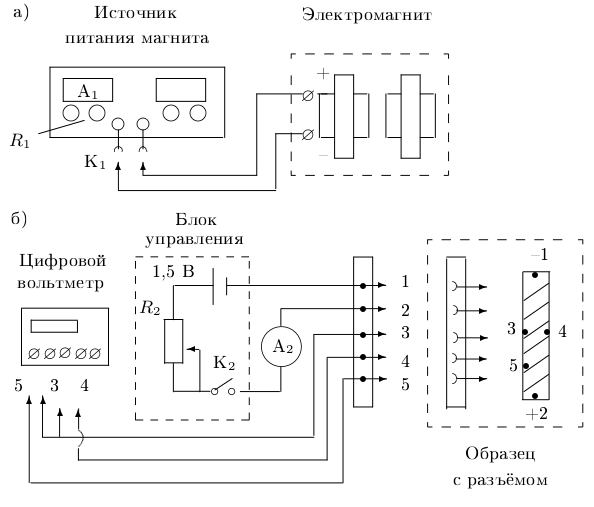
\includegraphics[scale=0.8]{pic1}}
 	\caption{Схема установки для исследования эффекта Холла в полупроводниках.}
\end{figure}

Схема установки для измерения ЭДС Холла представлена на рисунке \eqref{pic1}.

В зазоре электромагнита создаётся постоянное магнитное поле, величину которого можно менять с помощью регулятора $R_1$ источника питания электромагнита. Ток питания электромагнита измеряется амперметром $A_1$. Разьём $K_1$ позволяет менять направление тока в обмолках электромагнита.

Градуировка магнита проводится при помощи милливебермелра.

Образец из легированного германия, смонтированный в специальном держателе, подключается к источнику питания ($\simeq$ 1,5 В). При замыкании ключа $K_2$ вдоль длинной стороны образца течёт ток, величина которого регулируется реостатом $R_2$ и измеряется миллиамперметром $A_2$.

В образце с током, помещённом в зазор электромагнита, между контаклами 3 и 4 возникает разность потенциалов ($U_{34}$, которая измеряется с помощью цифрового вольтметра.

Иногда контакты 3 и 4 вследствие неточности поднайки не лежат на одной эквипотенциали, и тогда напряжение между ними связано не только с эффектом Холла, но и с омическим падением напряжения, вызванным протеканием основного тока через образец. Измеряемая разность потенциалов при одном направлении магнитного поля равна сумме ЭДС Холла и омического падения напряжения, а при друтом — их разности. В этом случае ЭДО Холла $\varepsilon_x$ может быть определена как половина алгебраической разности показаний вольтметра, полученных для двух противоположных направлений магнитного поля в зазоре. Знак измеряемого напряжения высвечивается на цифровом табло вольтметра.

Можно исключить влияние омического падения напряжения иначе, если при каждом токе через образец измерять напряжение между точками З и 4 в отсутствие магнитного поля. При фиксированном токе через образец это дополнительное к ЭДС Холла напряжение $U_0$ остаётся неизменным. От него следует (с учётом знака) отсчитывать величину ЭДС Холла:

\begin{equation}\label{eq1}
\varepsilon_x = U_{34} \pm U_0
\end{equation}

При таком способе измерения нет необходимости проводить повторные измерения с противоположным направлением магнитного поля.

По знаку $\varepsilon_x$ можно определить характер проводимости — электронный или дырочный. Для этого необходимо зналь направление тока в образце и направление магнитного поля.

Измерив ток I в образце и напряжение $U_{35}$ между контактами 3 и 5 в отсутствие магнитного поля, можно, зная параметры образца, рассчитать проводимость материала образца по формуле

\begin{equation}\label{eq2}
\sigma = \frac{I L_{35}}{U_{35} \textit{a l}}
\end{equation}

Где $L_{35}$ -- расстояние между контактами 3 и 5, \textit{a} -- толщина образца, \textit{l} -- его ширина.

\section{Ход работы.}

В работе предлагается исследовать зависимость ЭДС Холла от величины магнитного поля при различных токах через образец для определения константы Холла; определиль знак носителей заряда и проводимость материала образца.

1. Подготовим приборы к работе.

2. Проверим работу цепи питания образца. Ток через образец не должен
превышать 1 мА.

3. Проверим раболу цепи магнита. Определите диапазон изменения тока через магнит.

4. Прокалибруем электромагнит -- определите связь между индукцией В магнитного поля в зазоре электромагнита и током $I_m$ через обмотки магнита. Для этого с помощью милливеберметра снимем зависимость магнитного потока, $\Phi$ пронизывающего пробную катушку, находящуюся в зазоре, от тока $I_m$ ($\Phi = \text{BSN}$). Значение SN (произведение площади сечения контура катушки на число токов в ней) указано на держателе катушки.

5. Продевед измерение ЭДС Холла. Для этого втавим образец в зазор выключенного электромагнита и определим напряжение $U_0$ между холловскими контактами 3 и 4при минимальном токе через образец ($\simeq 0.2 \text{мА}$). Это напряжение $U_0$ вызвано несовершенством контактов 3, 4 и при фиксированном токе через образец остается неизменным. Значение $U_0$ с учетом значка следует принять за нулевое.

Включим электромагнит и снимем зависимость напряжения $U_{34}$ от тока $I_m$ через обмотки магнита при фиксированном токе через образец.

Проведем измерения $U_{34} = \textit{f }(I_m)$ при постоянном токе через образец для 6-8 его значений в интервале 0.2-1 мА. При каждом новом значении тока через образец величина $U_0$ будет иметь свое значение.

При максимальном токе через образец ($\simeq 1$ мА) $U = \textit{f }(I_m)$ при другом направлении магнитного поля.

6. Определим знак носителей в образце. Для этого необходимо знать направление тока через образец, направление магнитного поля и знак ЭДС Холла.

Направление тока в образце показано знаками «+» и «-» на рисунке \eqref{pic1}. Направление тока в обмотках электромагнита при установке разъёма $K_1$ в положение I показано стрелкой на торце магнита.

Сфотографируем образец. Укажем на рисунке направления тока, магнитного поля и отклонение носителей. По знаку ($\pm$) на клеммах цифрового вольтметра определите характер проводимости.

7. Для определение удельной проводимости удалим держатель с образцом из зазора. Подлкючим к клеммам «$H_x$» и «$L_x$» вольтметра поленциальные концы 3 и 5. Измерим падение напряжения между ними при токе через образец 1 мА.

8. Запишем характеристики приборов и параметры образца $L_{35}$, \textit{a, l}, указанные на держателе.

\section{Обработка результатов.}


\end{document} % конец документа